\documentclass[aspectratio=169]{beamer}
\usepackage{fontspec}
\setmainfont{Times New Roman}
\setsansfont{Calibri}
\setmonofont{Consolas}
\usepackage{polyglossia}
\setmainlanguage{ukrainian}
\setotherlanguage{english}
\usepackage{graphicx}
\usepackage{booktabs}
\usepackage{amsmath}
\usepackage{tikz}
\usetikzlibrary{arrows.meta, positioning, shapes.geometric}

\graphicspath{{figures/}}

% --- Theme ---
\usetheme{Madrid}
\usecolortheme{whale}
\setbeamertemplate{navigation symbols}{}
\setbeamertemplate{footline}[frame number]
\setbeamerfont{frametitle}{size=\large}

\title{Дослідження якості україно-англійського\\автоматичного перекладу мовлення}
\subtitle{Семантична точність та міжфразова когерентність}
\author{Нанаров Ілля Олександрович}
\institute{НаУКМА, факультет інформатики\\Кафедра математики\\[0.3em]
Керівник: Іванюк А.\,О.}
\date{2025}

\begin{document}

% ===== TITLE =====
\begin{frame}
\titlepage
\end{frame}

% ===== АКТУАЛЬНІСТЬ =====
\begin{frame}{Актуальність}
\begin{itemize}
    \item Переклад мовлення --- задача на перетині ASR та MT
    \item Пара \textbf{uk\,$\to$\,en}: складна морфологія, обмежені паралельні корпуси
    \item Більшість досліджень оцінюють ASR та MT \textbf{окремо}, ігноруючи каскадний ефект
    \item Комплексне дослідження для пари uk--en з аналізом каскадного ефекту та порівнянням із LLM \textbf{раніше не проводилось}
\end{itemize}
\end{frame}

% ===== МЕТА =====
\begin{frame}{Мета та завдання}
\textbf{Мета:} кількісне оцінювання якості україно-англійського автоматичного перекладу мовлення

\vspace{0.5em}
\textbf{Завдання:}
\begin{enumerate}
    \item Сформувати корпус дослідження
    \item Обрати систему метрик (BLEU, BERTScore, METEOR)
    \item Оцінити якість ASR (Whisper) та MT (OPUS-MT)
    \item Дослідити каскадний ефект (ASR$\to$MT)
    \item Провести ручну анотацію помилок
    \item Порівняти OPUS-MT з LLM-системами
\end{enumerate}
\end{frame}

% ===== КОРПУС =====
\begin{frame}{Корпус дослідження}
\begin{columns}[T]
\begin{column}{0.55\textwidth}
\begin{itemize}
    \item \textbf{Джерело:} звернення з president.gov.ua
    \item \textbf{Обсяг:} 7 записів $\to$ 12 сегментів
    \item \textbf{Тривалість:} $\approx$45 хвилин
    \item \textbf{Домен:} політичний дискурс
    \item Сегментація на основі пауз (3--5 хв)
    \item Ручна корекція транскрипцій
    \item Референсні переклади (LLM + ручна верифікація)
\end{itemize}
\end{column}
\begin{column}{0.42\textwidth}
\small
\begin{tabular}{lcc}
\toprule
\textbf{Запис} & \textbf{Сегм.} & \textbf{Трив.} \\
\midrule
В Еміратах & 2 & 8 хв \\
Діалог з Амер. & 2 & 8 хв \\
Знаємо, що... & 2 & 7 хв \\
Командна ланка & 1 & 4 хв \\
Наша стратегія & 2 & 7 хв \\
Отримуємо... & 1 & 4 хв \\
Поведінка & 2 & 7 хв \\
\midrule
\textbf{Разом} & \textbf{12} & \textbf{45 хв} \\
\bottomrule
\end{tabular}
\end{column}
\end{columns}
\end{frame}

% ===== АРХІТЕКТУРА =====
\begin{frame}{Архітектура pipeline}
\begin{center}
\begin{tikzpicture}[
    node distance=1.4cm,
    box/.style={draw, rounded corners, fill=blue!10, minimum height=1.1cm, minimum width=2.6cm, align=center, font=\footnotesize},
    arrow/.style={-{Stealth[length=3mm]}, thick},
    label/.style={font=\footnotesize, text=gray}
]
\node[box, fill=orange!15] (audio) {Аудіо\\(WAV, 44.1 kHz)};
\node[box, right=of audio, fill=blue!15] (asr) {ASR\\Whisper medium\\769M параметрів};
\node[box, right=of asr, fill=green!15] (mt) {MT\\OPUS-MT\\74M параметрів};
\node[box, right=of mt, fill=purple!15] (out) {Переклад\\англійською};

\draw[arrow] (audio) -- (asr) node[midway, above, label] {$x(t)$};
\draw[arrow] (asr) -- (mt) node[midway, above, label] {$\hat{y}$ (укр.)};
\draw[arrow] (mt) -- (out) node[midway, above, label] {$\hat{z}$ (eng.)};

\node[box, below=1.2cm of mt, fill=red!10] (llm) {LLM (додатково)\\GPT-4o / Claude / Gemini};
\draw[arrow, dashed] (asr) |- (llm);
\draw[arrow, dashed] (llm) -| (out);
\end{tikzpicture}
\end{center}

\vspace{0.3em}
\begin{columns}[T]
\begin{column}{0.48\textwidth}
\small
\textbf{Переваги каскаду:}\\
модульність, інтерпретованість,\\покомпонентний аналіз помилок
\end{column}
\begin{column}{0.48\textwidth}
\small
\textbf{Продуктивність:}\\
RTF = 0,26$\times$ (без GPU)\\
$\approx$4$\times$ швидше за реальний час
\end{column}
\end{columns}
\end{frame}

% ===== МЕТРИКИ =====
\begin{frame}{Система метрик}
\begin{center}
\begin{tabular}{lll}
\toprule
\textbf{Аспект} & \textbf{Метрика} & \textbf{Що вимірює} \\
\midrule
Якість ASR & WER, CER & Помилки розпізнавання \\
\addlinespace
Лексичний збіг & BLEU & Збіг $n$-грам з референсом \\
Семантична подібність & BERTScore & Косинусна подібність ембедингів \\
Морфологічний збіг & METEOR & Стемінг + синоніми + порядок \\
\addlinespace
Ручна анотація & MQM & Пропуски / спотворення / додавання \\
Когерентність & Експертна оцінка & Зв'язність між сегментами (1--5) \\
\bottomrule
\end{tabular}
\end{center}
\end{frame}

% ===== РЕЗУЛЬТАТИ ASR =====
\begin{frame}{Результати ASR (Whisper medium)}
\begin{columns}[T]
\begin{column}{0.45\textwidth}
\begin{center}
\large
\textbf{WER = 8,62\%}\\[0.3em]
\textbf{CER = 2,10\%}\\[0.5em]
\normalsize
\textit{(типово 10--15\% для укр.)}
\end{center}

\vspace{0.5em}
\small
Розподіл помилок:
\begin{itemize}
    \item Заміни: 271 (82,6\%)
    \item Видалення: 38 (11,6\%)
    \item Вставки: 19 (5,8\%)
\end{itemize}

Проблемні категорії: власні назви, географічні назви, абревіатури
\end{column}
\begin{column}{0.53\textwidth}
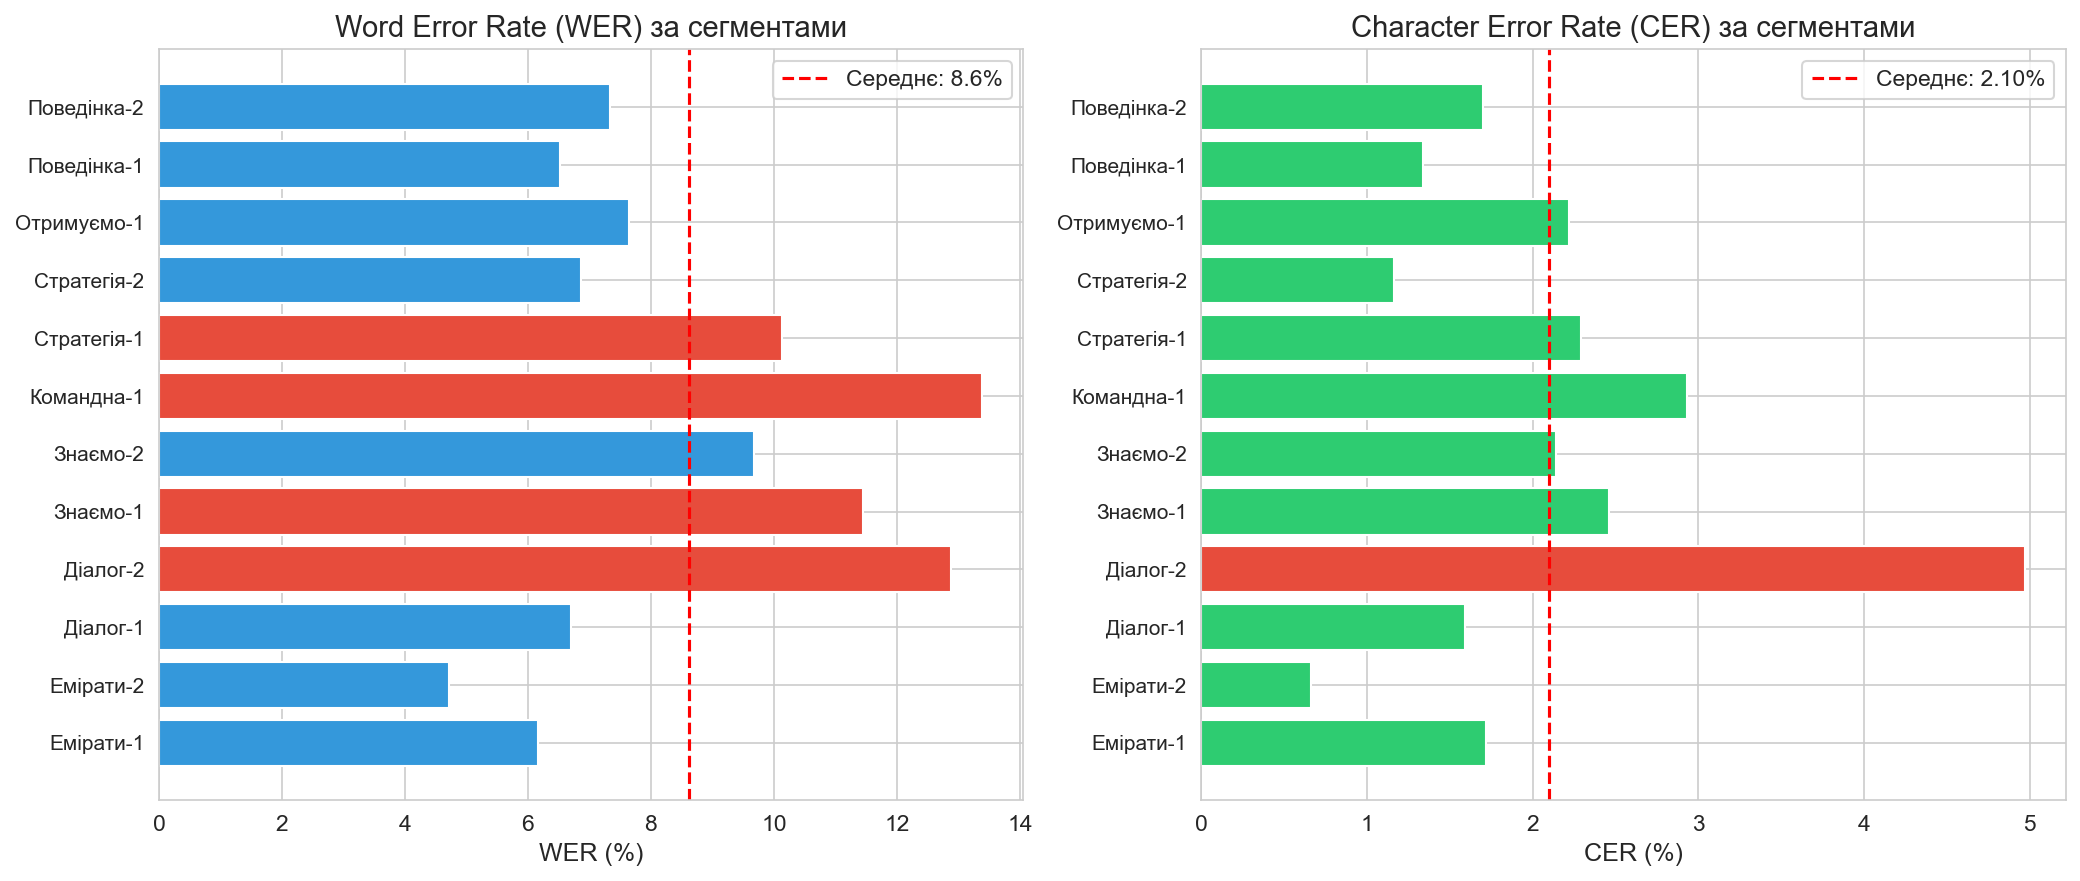
\includegraphics[width=\textwidth]{figures/asr_metrics_by_segment.png}
\end{column}
\end{columns}
\end{frame}

% ===== РЕЗУЛЬТАТИ MT =====
\begin{frame}{Результати MT (OPUS-MT)}
\begin{columns}[T]
\begin{column}{0.45\textwidth}
\begin{center}
\begin{tabular}{lc}
\toprule
\textbf{Метрика} & \textbf{Середнє} \\
\midrule
BLEU & 23,12 \\
BERTScore-F1 & 0,397 \\
METEOR & 0,452 \\
\bottomrule
\end{tabular}
\end{center}

\vspace{0.5em}
\small
\begin{itemize}
    \item BLEU 23 --- типовий для uk$\to$en
    \item Придатний для пост-редагування
    \item Найгірший сегмент: BLEU = 12,37 (висока щільність власних назв)
\end{itemize}
\end{column}
\begin{column}{0.53\textwidth}
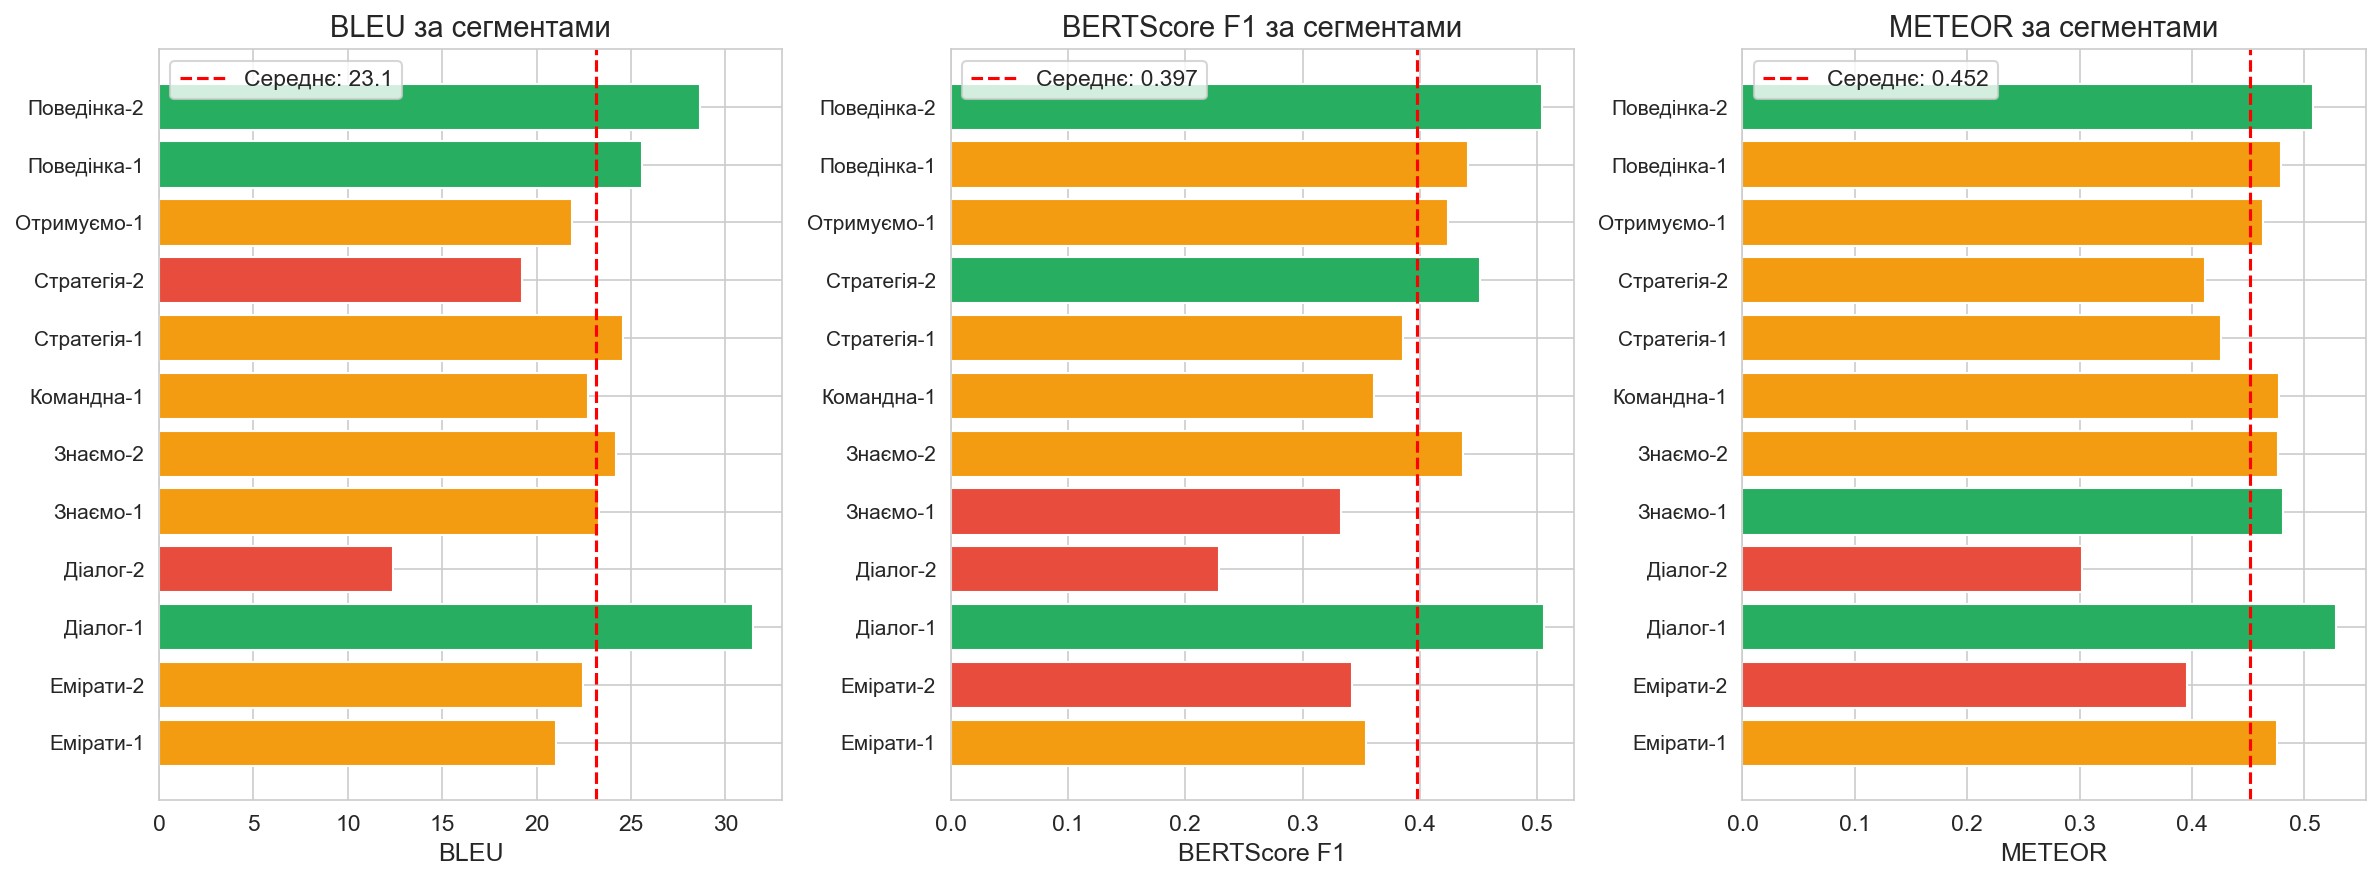
\includegraphics[width=\textwidth]{figures/mt_metrics_by_segment.png}
\end{column}
\end{columns}
\end{frame}

% ===== РУЧНЕ ОЦІНЮВАННЯ =====
\begin{frame}{Ручне оцінювання: 114 помилок OPUS-MT}
\begin{columns}[T]
\begin{column}{0.48\textwidth}
\textbf{За типами:}
\begin{tabular}{lcc}
\toprule
Тип & К-сть & \% \\
\midrule
Спотворення & 91 & 79,8\% \\
Пропуски & 19 & 16,7\% \\
Додавання & 4 & 3,5\% \\
\bottomrule
\end{tabular}

\vspace{0.5em}
\textbf{Категорії спотворень:}
\begin{tabular}{lc}
\toprule
Категорія & \% \\
\midrule
Власні назви & 46,2\% \\
Географічні назви & 16,5\% \\
Семантичні & 15,4\% \\
Військова терм. & 13,2\% \\
\bottomrule
\end{tabular}
\end{column}
\begin{column}{0.50\textwidth}
\textbf{Критичні помилки (7):}
\small
\begin{tabular}{ll}
\toprule
\textbf{MT} & \textbf{Референс} \\
\midrule
20,000 dollars & 20,000 hryvnias \\
our killers & our warriors \\
Crete & Kryvyi Rih \\
Crimea & Kryvyi Rih \\
sewers & resilience \\
\bottomrule
\end{tabular}

\vspace{0.5em}
\textbf{Когерентність:} 3,2 / 5\\
\small Тематика збережена, але непослідовність у передачі власних назв
\end{column}
\end{columns}
\end{frame}

% ===== КАСКАДНИЙ ЕФЕКТ =====
\begin{frame}{Каскадний ефект: помилки ASR $\to$ якість MT}
\begin{columns}[T]
\begin{column}{0.48\textwidth}
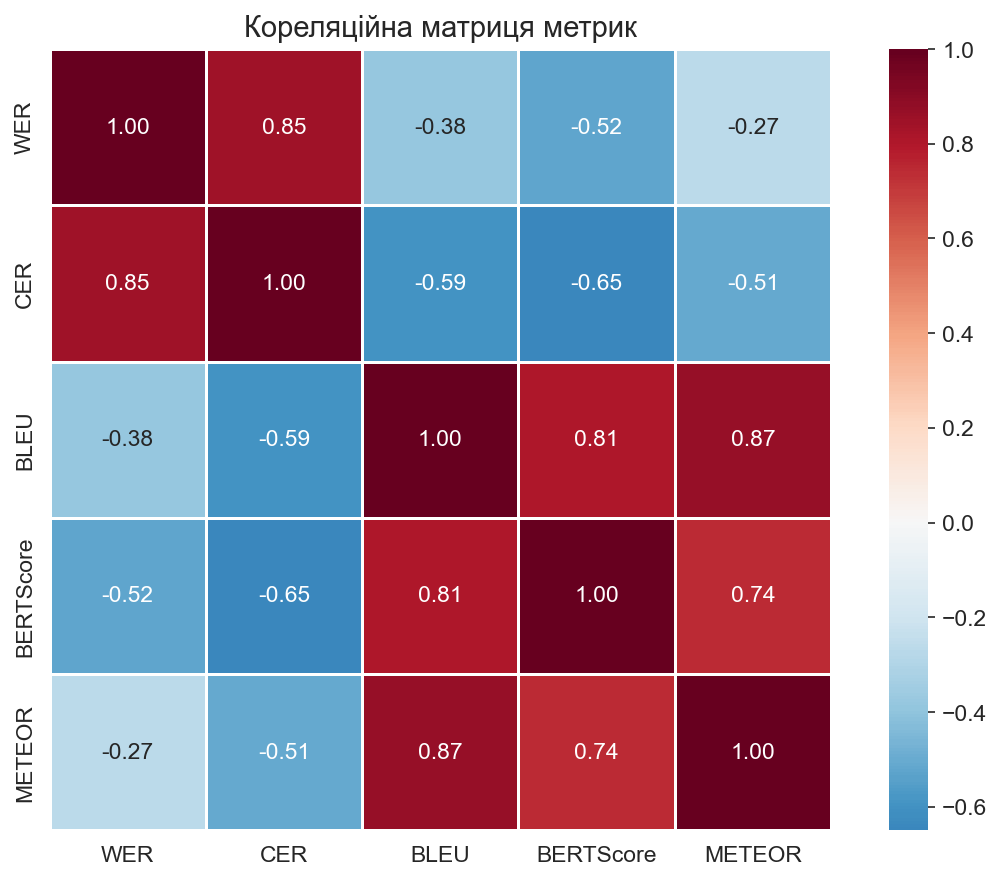
\includegraphics[width=\textwidth]{figures/correlation_heatmap.png}
\end{column}
\begin{column}{0.50\textwidth}
\textbf{Статистично значущі кореляції:}

\vspace{0.5em}
\begin{tabular}{lcc}
\toprule
\textbf{Пара} & $r$ & $p$ \\
\midrule
CER $\leftrightarrow$ BLEU & $-0,59$ & 0,042 \\
CER $\leftrightarrow$ BERTScore & $-0,65$ & 0,022 \\
\bottomrule
\end{tabular}

\vspace{0.8em}
\begin{itemize}
    \item CER впливає сильніше, ніж WER
    \item Помилки у власних назвах каскадно погіршують переклад
    \item OPUS-MT не має механізму корекції вхідних помилок
\end{itemize}
\end{column}
\end{columns}
\end{frame}

% ===== LLM =====
\begin{frame}{Порівняння з LLM-системами}
\begin{columns}[T]
\begin{column}{0.48\textwidth}
\begin{center}
\begin{tabular}{lccc}
\toprule
\textbf{Модель} & \textbf{BLEU} & \textbf{BERT} & \textbf{MET.} \\
\midrule
OPUS-MT & 23,1 & 0,40 & 0,45 \\
\textbf{GPT-4o} & \textbf{57,0} & 0,73 & 0,75 \\
Claude S.~4 & 55,5 & 0,71 & 0,73 \\
Gemini 2.0 & 56,9 & \textbf{0,74} & \textbf{0,75} \\
\bottomrule
\end{tabular}
\end{center}

\vspace{0.3em}
\small
Покращення LLM vs OPUS-MT:
\begin{itemize}
    \item BLEU: \textbf{+147\%}
    \item BERTScore: \textbf{+82\%}
    \item METEOR: \textbf{+65\%}
\end{itemize}
$p < 0,001$ (Манна-Уітні)
\end{column}
\begin{column}{0.50\textwidth}
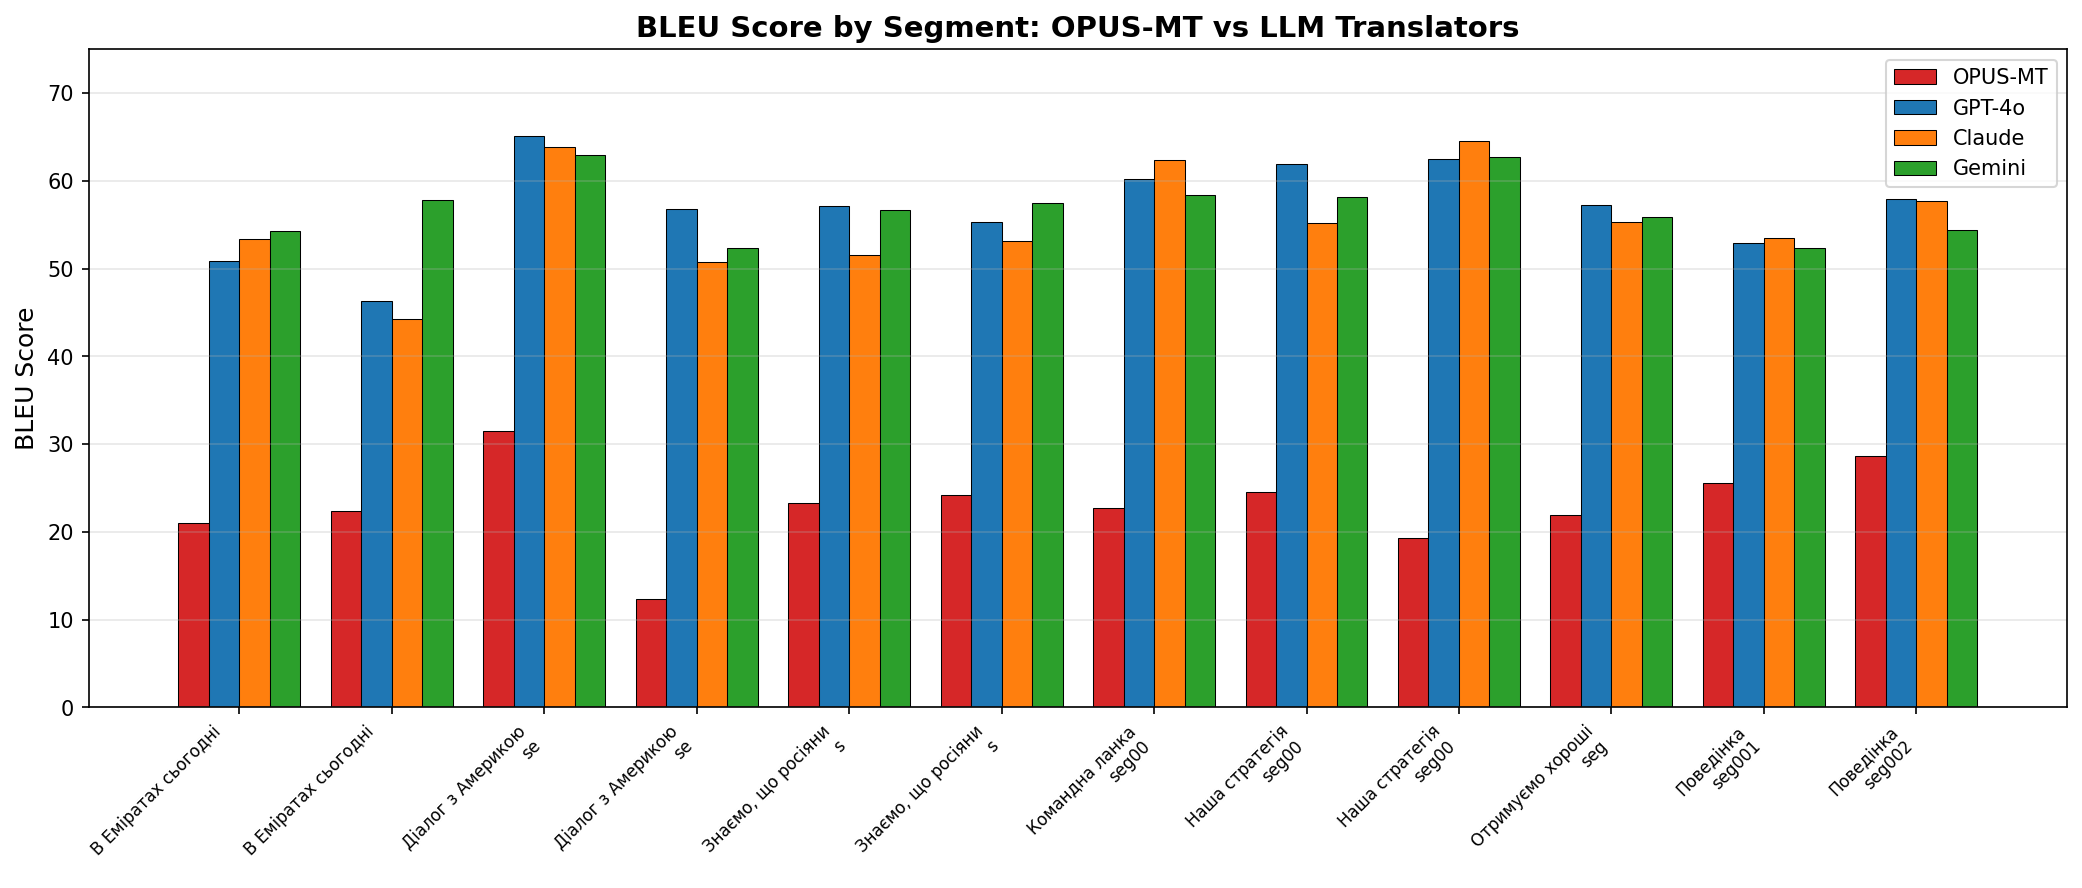
\includegraphics[width=\textwidth]{figures/llm_bleu_by_segment.png}

\vspace{0.3em}
\small
\textbf{Ключова перевага LLM:}\\
коригують помилки ASR у власних назвах завдяки контекстуальним знанням

\vspace{0.3em}
\textbf{Обмеження:} вища латентність,\\
залежність від API, вартість
\end{column}
\end{columns}
\end{frame}

% ===== LLM ПРИКЛАДИ =====
\begin{frame}{LLM: корекція помилок ASR}
\begin{center}
\begin{tabular}{llll}
\toprule
\textbf{ASR (Whisper)} & \textbf{OPUS-MT} & \textbf{GPT-4o} & \textbf{Референс} \\
\midrule
Рустему Міров & Rustema Mirov & Rustem Umerov & Rustem Umerov \\
Кривирі & Crete & Kryvyi Rih & Kryvyi Rih \\
генерал Гнатов & General Gnatov & General Hnatov & General Hnatov \\
ГУР & MBI & HUR (Def. Intel.) & HUR \\
\bottomrule
\end{tabular}
\end{center}

\vspace{0.5em}
LLM здатні:
\begin{enumerate}
    \item Розпізнавати та коригувати помилки ASR у власних назвах
    \item Застосовувати стандартну транслітерацію українських топонімів
    \item Правильно розшифровувати українські абревіатури
\end{enumerate}
\end{frame}

% ===== ВИСНОВКИ =====
\begin{frame}{Висновки}
\begin{enumerate}
    \item \textbf{ASR:} Whisper medium --- WER = 8,62\%, краще за типові 10--15\%

    \item \textbf{MT (OPUS-MT):} BLEU = 23,12 --- типовий для uk$\to$en, придатний для пост-редагування

    \item \textbf{LLM:} BLEU = 55--57 (\textbf{+147\%}), $p < 0,001$; критично краща обробка власних назв

    \item \textbf{Каскадний ефект:} $r = -0,65$ для CER--BERTScore ($p = 0,022$) --- помилки ASR статистично значуще погіршують якість MT

    \item \textbf{Помилки:} 114 помилок, 79,8\% --- спотворення (46,2\% у власних назвах)

    \item \textbf{Практична рекомендація:} LLM для офлайн-перекладу,\\OPUS-MT для real-time з пост-редагуванням
\end{enumerate}
\end{frame}

% ===== ДЯКУЮ =====
\begin{frame}
\begin{center}
\vspace{2cm}
{\Huge Дякую за увагу!}\\[1.5cm]
{\large Нанаров Ілля Олександрович}\\[0.5em]
{\normalsize illya.nanarov@ukma.edu.ua}\\[1em]
{\small Код та дані: github.com/IllyaMoore/ukrainian-speech-translation-research}
\end{center}
\end{frame}

\end{document}
